\section{Buffers}
在本章中,我们将学习Buffer抽象。 我们在上一章中了解了统一共享内存(USM),这是一种基于指针的数据管理策略。 
USM 迫使我们思考内存存放在哪里以及什么应该在哪里访问。 Buffer抽象是一个更高级别的模型,它向程序员隐藏了这一点。 
Buffer只是代表数据,运行时的工作就是管理数据在内存中的存储和移动方式。

本章介绍了管理数据的另一种方法。 Buffer和 USM 之间的选择通常取决于个人喜好和现有代码的风格,
并且应用程序可以自由地混合和匹配这两种风格以表示应用程序中的不同数据。

USM 只是公开不同的内存抽象。 USM 有指针,Buffer是更高级别的抽象。 
Buffer的抽象级别允许在应用程序内的任何设备上使用其中包含的数据,其中运行时管理使该数据可用所需的任何内容。 
USM 基于指针的模型可能更适合使用基于指针的数据结构(例如链表、树或其他结构)的应用程序。 
将Buffer改造为已经使用指针的现有代码也可能更加棘手。 
但是,Buffer保证可以在系统中的每个设备上工作,而某些设备可能不支持特定(或任何)USM 模式。 
选择很好,所以让我们深入研究Buffer。

我们将更仔细地了解Buffer是如何创建和使用的。 如果不讨论访问器,对Buffer的讨论就不完整。 
虽然Buffer抽象了我们在程序中表示和存储数据的方式,但我们并不直接使用Buffer访问数据。 
相反,我们使用访问器对象来通知运行时我们打算如何使用正在访问的数据,并且访问器与任务图中强大的数据依赖机制紧密耦合。 
在我们介绍了可以使用Buffer执行的所有操作之后,我们还将探索如何在程序中创建和使用访问器。


\subsection{Buffers}
Buffer是数据的高级抽象。 Buffer不一定绑定到单个位置或虚拟内存地址。 
事实上,运行时可以自由地使用内存中的许多不同位置(甚至跨不同的设备)来表示Buffer,
但运行时必须确保始终为我们提供一致的数据视图。 Buffer可以在主机和任何设备上访问。

\begin{figure}[H]
	\centering
	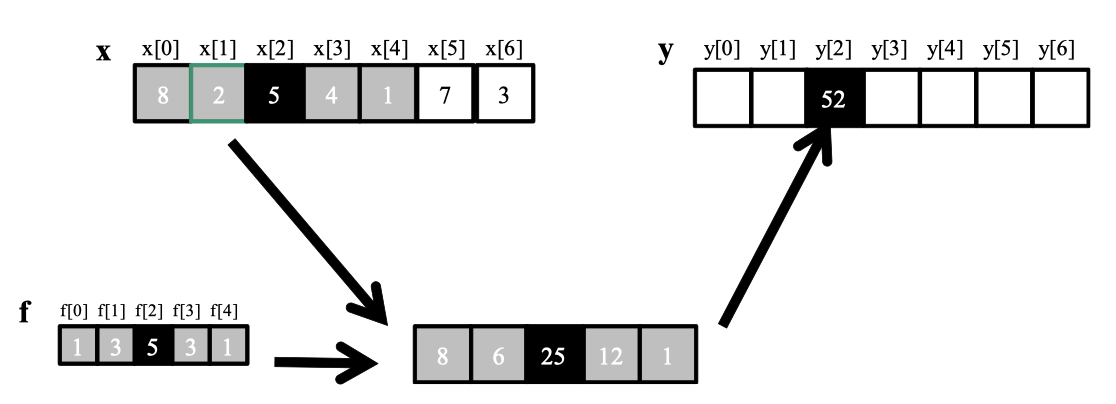
\includegraphics[width=0.9\textwidth]{figs/F7.1.png}
	\caption{\textit{Buffer 类定义 }}
\end{figure}

Buffer类是一个具有三个模板参数的模板类,如图 7-1 所示。 第一个模板参数是Buffer将包含的对象的类型。 
此类型必须是设备可复制的,这扩展了 C++ 定义的普通可复制的概念。 
可简单复制的类型可以安全地逐字节复制,而无需使用任何特殊的复制或移动构造函数。 
设备可复制类型将此概念递归地扩展到某些 C++ 类型,例如 std::pair 或 std::tuple。 
下一个模板参数是描述Buffer维数的整数。 最后的模板参数是可选的,默认值通常是使用的值。 
此参数指定一个 C++ 样式的分配器类,用于在主机上执行Buffer所需的任何内存分配。 
首先,我们将研究创建Buffer对象的多种方法。

\subsubsection{Buffer创建}
在下图中,我们展示了创建Buffer对象的几种方法。 让我们浏览一下示例并查看每个实例。

\begin{figure}[H]
	\centering
	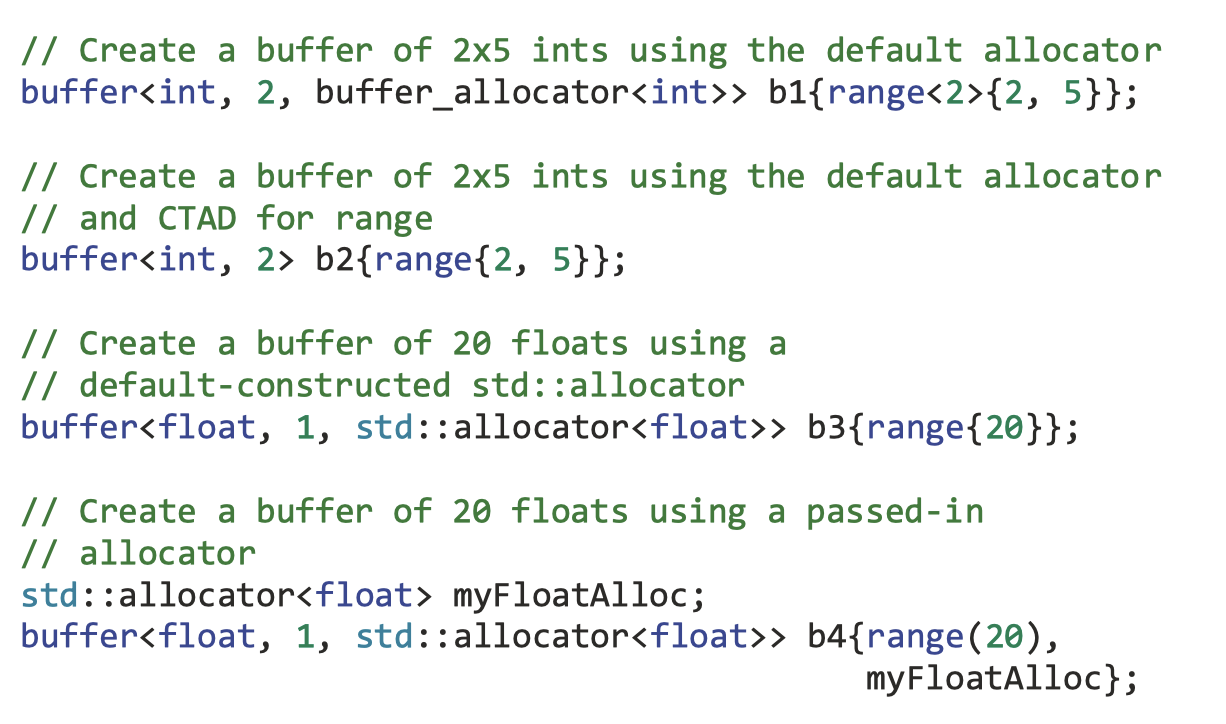
\includegraphics[width=0.9\textwidth]{figs/F7.2.png}
	\caption{\textit{创建Buffer,第一部分 }}
\end{figure}

我们在图 7-2 中创建的第一个Buffer b1 是一个包含 10 个整数的二维Buffer。 
我们显式传递所有模板参数,甚至显式传递 buffer\_allocator<T> 的默认值作为分配器类型。 
由于 buffer\_allocator 也是模板化类型,因此我们必须显式地专门化它,
就像通过指定 buffer\_allocator<int> 来专门化Buffer一样。 然而,使用现代 C++,我们可以更简洁地表达这一点。 
Buffer b2 也是使用默认分配器的十个整数的二维Buffer。 
这里我们利用 C++17 的类模板参数推导(CTAD)来自动推断模板参数。 
CTAD 是一个全有或全无的工具,它必须要么推断出类的每个模板参数,要么不推断出其中任何一个。 
在本例中,我们利用这样一个事实:我们用一个带有两个参数的范围来初始化 b2 来推断它是一个二维范围。 
分配器模板参数有一个默认值,因此我们在创建Buffer时不需要显式列出它。

使用Buffer b3,我们创建一个 20 个浮点数的Buffer,并使用默认构造的 std::allocator 来分配主机上任何必要的内存。 
当将自定义分配器类型与Buffer一起使用时,我们通常希望将实际的分配器对象传递给Buffer来使用,而不是默认构造的分配器对象。 
Buffer b4 展示了如何执行此操作,在调用其构造函数的范围之后获取分配器对象。

对于示例中的前四个Buffer,我们让Buffer分配它需要的任何内存,并且在创建数据时不使用任何值初始化该数据。 
使用Buffer来有效包装现有的 C++ 分配是一种常见模式,这些分配可能已经使用数据进行了初始化。 
我们可以通过将初始值源传递给Buffer构造函数来做到这一点。 这样做可以让我们做几件事,我们将在下一个示例中看到。

\begin{figure}[H]
	\centering
	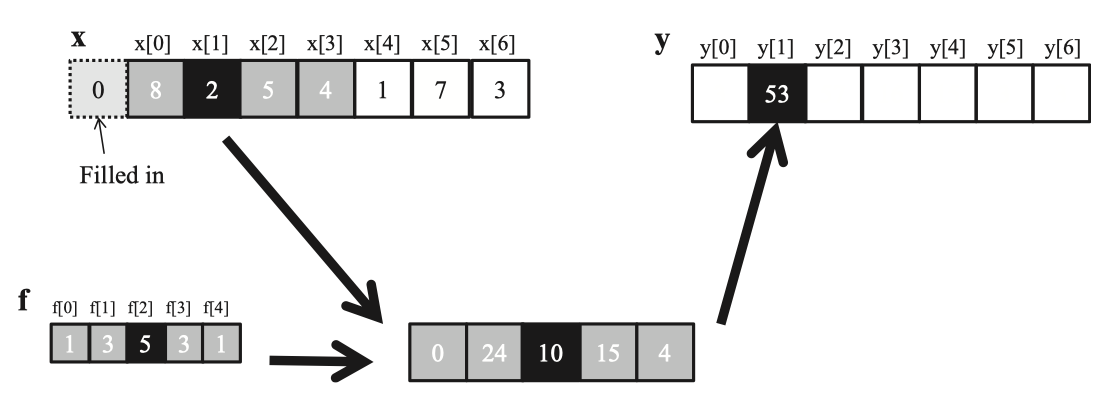
\includegraphics[width=0.9\textwidth]{figs/F7.3.png}
	\caption{\textit{创建Buffer,第二部分 }}
\end{figure}

在图 7-3 中,Buffer b5 创建一个包含四个双精度数的一维Buffer。 
除了指定Buffer大小的范围之外,我们还将指向 C 数组 myDoubles 的主机指针传递给Buffer构造函数。 
这里我们可以充分利用 CTAD 来推断Buffer的所有模板参数。 
我们传递的主机指针指向双精度数,它为我们提供了Buffer的数据类型。 
维数是从一维范围自动推断的,一维范围本身是推断出来的,因为它仅由一个数字创建。 
最后,使用默认分配器,因此我们不必指定它。

传递主机指针有一些我们应该注意的后果。 
通过传递指向主机内存的指针,我们向运行时保证在Buffer的生命周期内不会尝试访问主机内存。 
这不是(也不能)由 SYCL 实施强制执行。我们有责任确保我们不违反本合同。 
我们不应该在Buffer处于活动状态时尝试访问此内存的原因之一是,Buffer可能会选择使用主机上的不同内存来表示Buffer内容,
这通常是出于优化原因。 如果这样做,这些值将从主机指针复制到这个新内存中。 
如果后续Kernel修改Buffer,则原始主机指针将不会反映更新的值,直到某些指定的同步点。 
我们将在本章后面详细讨论数据何时写回到主机指针。

Buffer b6 与Buffer b5 非常相似,但有一个主要区别。 这次,我们使用指向 const double 的指针来初始化Buffer。 
这意味着我们只能通过主机指针读取值而不能写入它们。 
然而,本例中Buffer的类型仍然是 double,而不是 const double,因为推导指南没有考虑常量性。 
这意味着Buffer可以由Kernel写入,但在Buffer过期后我们必须使用不同的机制来更新主机(本章稍后将介绍)。

Buffer也可以使用 C++ 共享指针对象进行初始化。 
如果我们的应用程序已经使用共享指针,这非常有用,因为这种初始化方法将正确计算引用并确保内存不会被释放。 
Buffer b7 创建一个包含单个整数的Buffer,并使用共享指针对其进行初始化。

\begin{figure}[H]
	\centering
	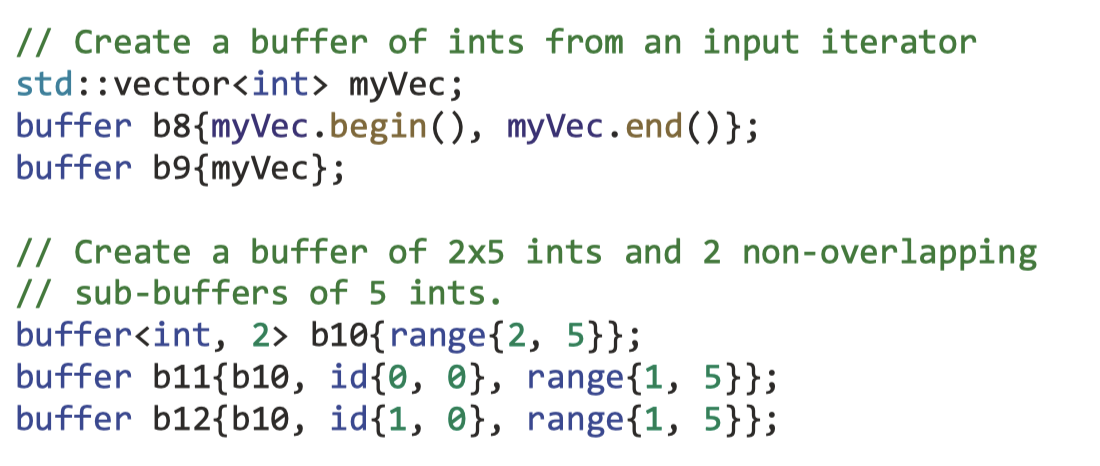
\includegraphics[width=0.9\textwidth]{figs/F7.4.png}
	\caption{\textit{创建Buffer,第三部分 }}
\end{figure}

容器通常用于现代 C++ 应用程序,示例包括 std::array、std::vector、std::list 或 std::map。 
我们可以通过两种不同的方式使用容器初始化一维Buffer。 第一种方式,如图 7-4 中的Buffer b8 所示,使用输入迭代器。 
我们将两个迭代器传递给Buffer构造函数,而不是主机指针,一个代表数据的开头,另一个代表数据的结尾。 
Buffer的大小计算为通过递增起始迭代器直到等于结束迭代器而返回的元素数。 
这对于实现 C++ InputIterator 接口的任何数据类型都很有用。 
如果为Buffer提供初始值的容器对象也是连续的,那么我们可以使用更简单的形式来创建Buffer。 
Buffer b9 只需将向量传递给构造函数即可从向量创建Buffer。 
Buffer的大小由用于初始化它的容器的大小决定,Buffer数据的类型来自容器数据的类型。 
使用这种方法创建Buffer很常见,并且建议在 std::vector 和 std::array 等容器中使用这种方法。

Buffer创建的最后一个示例说明了Buffer类的另一个功能。 可以创建一个子Buffer,它是一个Buffer的另一个Buffer的视图。
 子Buffer需要三件事:对父Buffer的引用、基本索引和子Buffer的范围。 无法从子Buffer创建子Buffer。 
 可以从同一个Buffer创建多个子Buffer,并且它们可以自由重叠。 
 Buffer b10 的创建方式与Buffer b2 完全相同,Buffer b2 是一个二维整数Buffer,每行有 5 个整数。 
 接下来,我们从Buffer b10 创建两个子Buffer,子Buffer b11 和 b12。 
 子Buffer b11 从索引 (0,0) 开始,包含第一行中的每个元素。 
 类似地,子Buffer b12 从索引 (1,0) 开始,包含第二行中的每个元素。 
 这会产生两个不相交的子Buffer。 由于子Buffer不重叠,因此不同的Kernel可以同时对不同的子Buffer进行操作,
 但我们将在下一章中详细讨论调度执行图和依赖关系。

\subsubsection{Buffer 属性}

\begin{figure}[H]
	\centering
	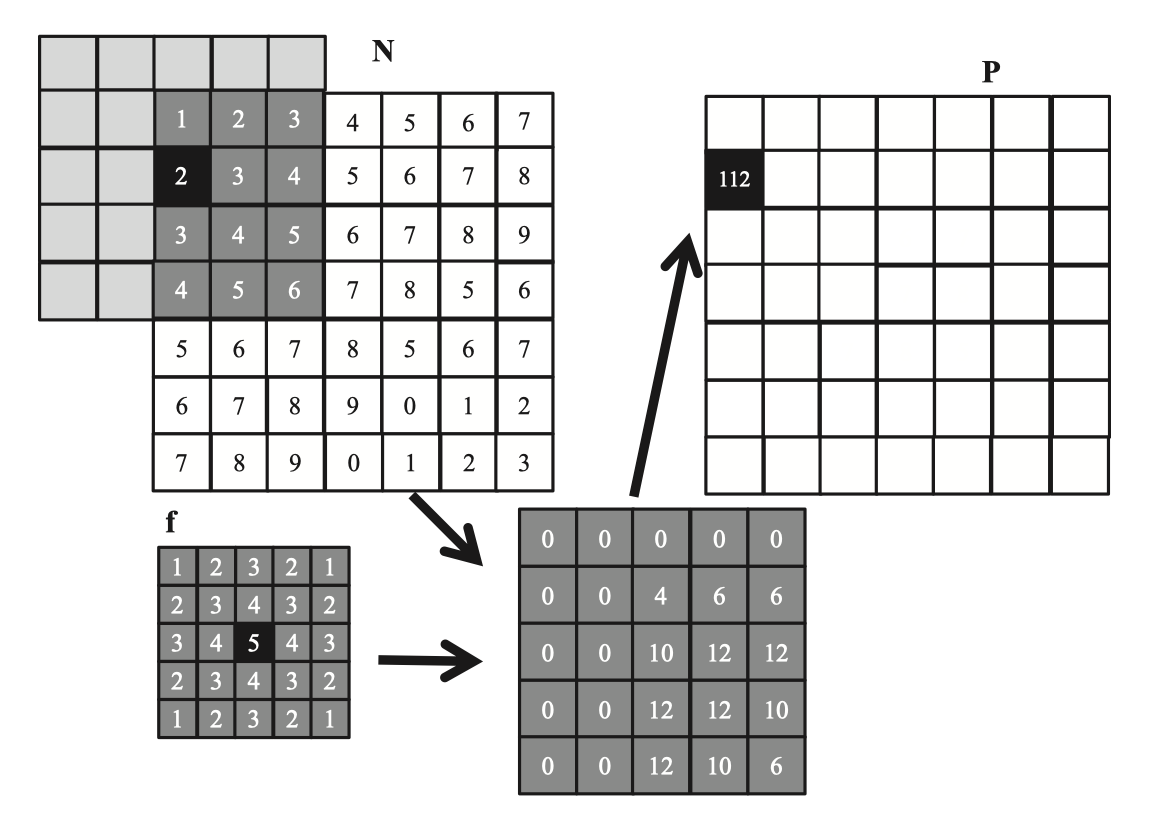
\includegraphics[width=0.9\textwidth]{figs/F7.5.png}
	\caption{\textit{Buffer属性 }}
\end{figure}

还可以使用改变其行为的特殊属性来创建Buffer。 
在图 7-5 中,我们将通过一个示例介绍三个不同的可选Buffer属性,并讨论如何使用它们。 
请注意,这些属性在大多数代码中相对不常见。

\paragraph{use\_host\_ptr}

在Buffer创建期间可以选择指定的第一个属性是 use\_host\_ptr。 
如果存在,此属性要求Buffer不在主机上分配任何内存,并且在Buffer构造中传递或指定的任何分配器都将被有效忽略。 
相反,Buffer必须使用传递给构造函数的主机指针指向的内存。 请注意,这并不要求设备使用相同的内存来保存Buffer的数据。 
设备可以自由地将Buffer的内容缓存在其附加内存中。 另请注意,仅当主机指针传递给构造函数时才可以使用此属性。 
当程序想要完全控制所有主机内存分配时,此选项非常有用,例如,它允许程序员尝试最小化应用程序的内存占用量。

在图 7-5 的示例中,我们创建了一个Buffer b,正如我们在前面的示例中看到的那样。 
接下来我们创建Buffer b1 并使用指向 myInts 的指针对其进行初始化。 
我们还传递了 use\_host\_ptr 属性,这意味着Buffer b1 将仅使用 myInts 指向的内存,
而不会在主机上分配任何额外的临时存储。

\paragraph{use\_mutex}

下一个属性 use\_mutex 涉及Buffer和主机代码之间的细粒度内存共享。 Buffer b2 是使用此属性创建的。 
该属性获取对互斥对象的引用,稍后可以从Buffer中查询该对象,如示例中所示。 
此属性还需要将主机指针传递给构造函数,它让运行时确定何时可以安全地通过提供的主机指针访问主机代码中的更新值。 
在运行时保证主机指针看到Buffer的最新值之前,我们无法锁定互斥体。 
虽然这可以与 use\_host\_ptr 属性结合使用,但这不是必需的。 
use\_mutex 是一种机制,允许主机代码在Buffer仍处于活动状态时访问Buffer内的数据,
并且无需使用主机访问器机制(稍后介绍)。 
一般来说,除非我们有特定原因使用互斥体,否则应首选主机访问器机制,
特别是因为无法保证成功锁定互斥体以及数据可供主机代码使用之前需要多长时间。

\paragraph{context\_bound}

在我们的示例中,最终属性显示在Buffer b3 的创建中。 
在这里,我们的 42 个整数的Buffer是使用 context\_bound 属性创建的。 
该属性采用对上下文对象的引用。 通常,Buffer可以在任何设备或上下文上自由使用。 
但是,如果使用此属性,则会将Buffer锁定到指定的上下文。 尝试在另一个上下文中使用Buffer将导致运行时错误。 
例如,这可以通过识别Kernel可能被提交到错误队列的情况来调试程序。 
实际上,我们并不期望在许多程序中看到此属性,
并且在任何上下文中的任何设备上访问Buffer的能力是Buffer抽象最强大的属性之一(此属性撤消了这一点)。

\subsubsection{我们可以用Buffer做什么?}
使用Buffer对象可以完成很多事情。 我们可以查询Buffer的特征,确定Buffer被破坏后是否以及在何处将任何数据写回主机内存,
或者将Buffer重新解释为具有不同特征的Buffer。 然而,不能做的一件事是直接访问Buffer表示的数据。 
相反,我们必须创建访问器对象来访问数据,我们将在本章后面学习所有这些内容。

可以查询Buffer的示例包括Buffer的范围、它表示的数据元素的总数以及存储其元素所需的字节数。 
我们还可以查询Buffer正在使用哪个分配器对象以及该Buffer是否是子Buffer。

当Buffer被破坏时更新主机内存是使用Buffer时需要考虑的一个重要方面。 
根据Buffer的创建方式,主机内存可能会也可能不会在Buffer销毁后使用计算结果进行更新。 
如果创建Buffer并从指向非常量数据的主机指针进行初始化,则当Buffer被销毁时,同一指针将使用最新数据进行更新。 
然而,还有一种方法可以更新主机内存,无论Buffer是如何创建的。 
set\_final\_data 方法是 buffer 的模板方法,它可以接受原始指针、C++ OutputIterator 或 std::weak\_ptr。 
当Buffer被破坏时,Buffer包含的数据将使用提供的位置写入主机。 
请注意,如果Buffer是从主机指针创建并初始化为非常量数据,则就像使用该指针调用 set\_final\_data 一样。 
从技术上讲,原始指针是 OutputIterator 的特殊情况。 
如果传递给 set\_final\_data 的参数是 std::weak\_ptr,则当指针已过期或已被删除时,数据不会写入主机。 
是否发生回写也可以通过set\_write\_back方法来控制。

\subsection{访问器}
Buffer表示的数据不能通过Buffer对象直接访问。 相反,我们必须创建允许我们安全访问Buffer数据的访问器对象。 
访问器通知运行时我们要在何处以及如何访问数据,从而允许运行时确保正确的数据在正确的时间位于正确的位置。 
这是一个非常强大的概念,特别是与部分基于数据依赖性来调度Kernel执行的任务图结合使用时。

访问器对象是从模板化访问器类实例化的。 该类有五个模板参数。 第一个参数是正在访问的数据的类型。 
这应该与相应Buffer存储的数据类型相同。 同样,第二个参数描述数据和Buffer的维度,默认值为 1。

\begin{figure}[H]
	\centering
	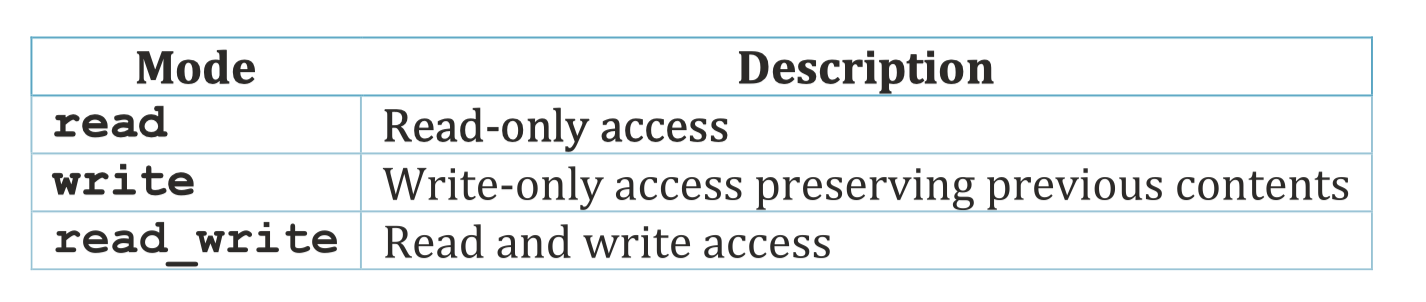
\includegraphics[width=0.9\textwidth]{figs/F7.6.png}
	\caption{\textit{访问模式 }}
\end{figure}

接下来的三个模板参数对于访问器来说是唯一的。 第一个是访问模式。 访问模式描述了我们打算如何在程序中使用访问器。 
图 7-6 列出了可能的模式。 我们将在第 8 章中了解如何使用这些模式来命令Kernel的执行和执行数据移动。
如果没有指定或自动推断,访问模式参数确实有一个默认值。 
如果我们没有另外指定,访问器将默认对非 const 数据类型使用 read\_write 访问模式,
对 const 数据类型默认使用 read 访问模式。 
这些默认值始终是正确的,但提供更准确的信息可能会提高运行时执行优化的能力。 
当开始应用程序开发时,简单地不指定访问模式是安全且简洁的,
然后我们可以根据应用程序的性能关键区域的分析来细化访问模式。

\begin{figure}[H]
	\centering
	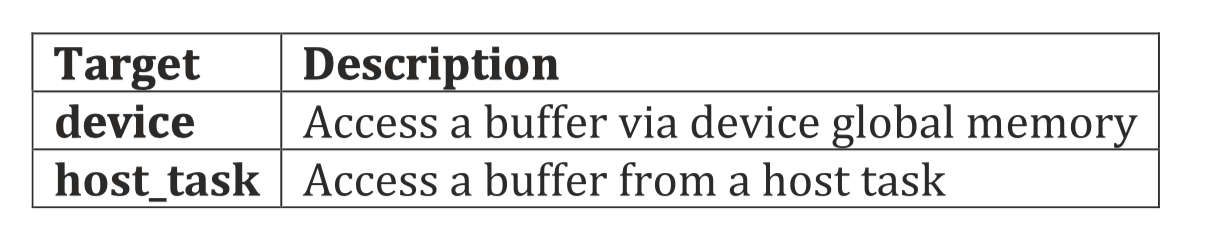
\includegraphics[width=0.9\textwidth]{figs/F7.7.png}
	\caption{\textit{访问目标 }}
\end{figure}

下一个模板参数是访问目标。 Buffer是数据的抽象,不描述数据的存储位置和方式。 
访问目标描述了我们正在访问数据的位置。 图 7-7 列出了两个可能的访问目标。

当使用带有 SYCL 的 C++ 时,只有两个目标:device 和 host\_task。 
默认模板值为 device,这意味着我们打算访问设备上的Buffer数据。 
这是合理的,因为访问器最常用于设备上的操作,例如Kernel或数据传输。 
另一个访问目标是 host\_task,当主机任务需要访问Buffer的数据时使用它。

设备可能有不同类型的可用存储器。 特别是,许多设备都具有某种快速本地内存,可以在工作组中的多个工作项之间共享。 
SYCL 的早期版本对本地内存有特殊的访问目标,但 SYCL 2020 以不同的方式处理它。 
我们将在第 9 章中学习如何使用工作组本地内存。
早期版本的 SYCL 还为主机提供了特殊的访问目标(在主机任务之外,这是 SYCL 2020 的新增功能)。 
它已被新的 host\_accessor 类取代,该类提供对主机代码中Buffer数据的访问。 
但是,访问将在 host\_accessor 的生命周期内保持有效。 
鉴于当 host\_accessor 有效时Buffer被锁定到主机,因此应特别注意限制 host\_accessor 对象的范围。

最终的模板参数控制访问器是否是占位符访问器。 
这不是程序员可能直接设置的参数,通常是通过使用构造函数调用来创建访问器来推断的。 
占位符访问器是在命令组外部声明的访问器,但旨在用于访问Kernel内设备上的数据。 
一旦我们查看了访问器创建的示例,我们就会明白占位符访问器与非占位符访问器的区别。

虽然可以使用其 get\_access 方法从Buffer对象中提取访问器,但直接创建(构造)它们更简单。 
这是我们将在接下来的示例中使用的样式,因为它非常易于理解并且紧凑。

\subsubsection{访问器创建}
\begin{figure}[H]
	\centering
	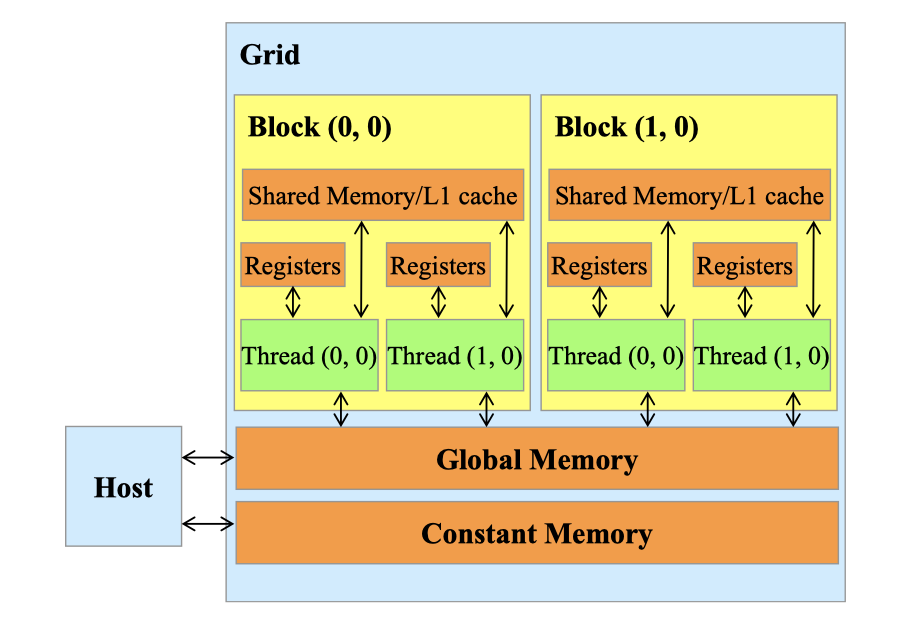
\includegraphics[width=0.9\textwidth]{figs/F7.8.png}
	\caption{\textit{创建简单的访问器 }}
\end{figure}

图 7-8 显示了一个示例程序,其中包含我们开始使用访问器所需的一切。 
在此示例中,我们有三个Buffer A、B 和 C。
我们提交到队列的第一个并行任务为每个Buffer创建访问器,并定义一个Kernel,该Kernel使用这些访问器用一些值初始化Buffer。 
每个访问器都是通过对其将访问的Buffer的引用以及我们提交到队列的命令组定义的处理程序对象来构造的。 
这有效地将访问器绑定到我们作为命令组的一部分提交的Kernel。 
常规访问器是设备访问器,因为默认情况下它们的目标是存储在设备内存中的全局Buffer。 这是最常见的用例。

我们提交的第二个任务还定义了三个Buffer访问器。 
然后,我们使用第二个Kernel中的这些访问器将Buffer A 和 B 的元素添加到Buffer C 中。
由于第二个任务操作的数据与第一个任务相同,因此运行时将在第一个任务完成后执行此任务。 
我们将在下一章详细了解这一点。

第三个任务展示了如何使用占位符访问器。 在我们创建Buffer之后,访问器 pC 在图 7-8 示例的开头声明。 
请注意,构造函数不会传递处理程序对象,因为我们没有要传递的处理程序对象。 
这让我们可以提前创建一个可重用的访问器对象。 但是,为了在Kernel中使用此访问器,我们需要在提交期间将其绑定到命令组。 
我们使用处理程序对象的 require 方法来完成此操作。 
一旦我们将占位符访问器绑定到命令组,我们就可以像使用任何其他访问器一样在Kernel中使用它。

最后,我们创建一个 host\_accessor 对象,以便在主机上读回计算结果。 
请注意,这与我们在Kernel中使用的类型不同。 
请注意,此示例中的主机访问器结果也不采用处理程序对象,因为我们再次没有要传递的处理程序对象。 
主机访问器的特殊类型还可以让我们消除它们与占位符的歧义。 
主机访问器的一个重要方面是,构造函数仅在数据可在主机上使用时完成,这意味着主机访问器的构造可能会花费很长时间。 
构造函数必须等待任何生成要复制的数据的Kernel完成执行以及复制本身完成。 
一旦主机访问器构建完成,就可以安全地使用它直接在主机上访问的数据,并且我们可以保证在主机上可以使用最新版本的数据。

虽然这个例子是完全正确的,但我们在创建访问器时并没有说明我们打算如何使用它们。 
相反,我们对Buffer中的非常量 int 数据使用默认访问模式,即 read\_write。 
这可能过于保守,并且可能会在操作之间产生不必要的依赖性或多余的数据移动。 
如果运行时有更多关于我们计划如何使用我们创建的访问器的信息,它可能会做得更好。 
然而,在我们讨论执行此操作的示例之前,我们应该首先介绍另一个工具 - 推导标签。

\begin{figure}[H]
	\centering
	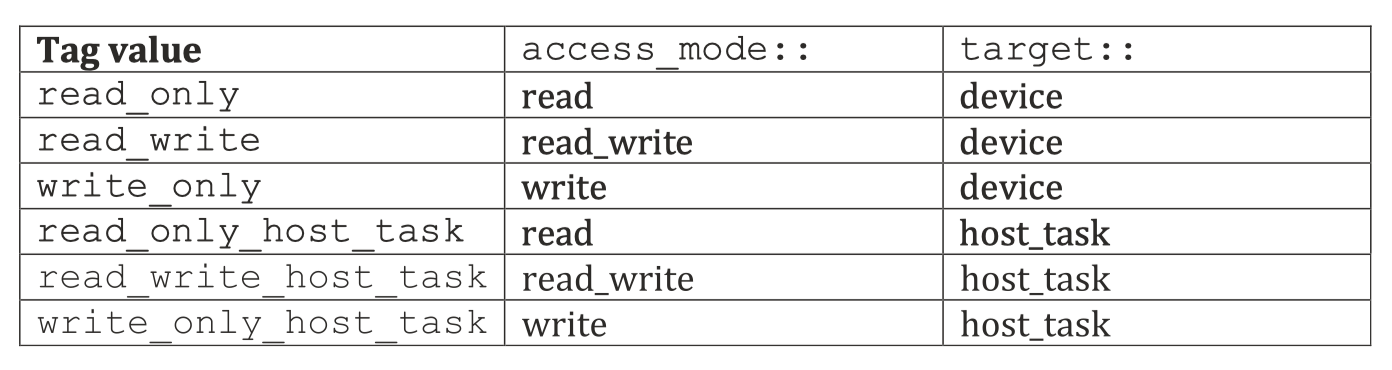
\includegraphics[width=0.9\textwidth]{figs/F7.9.png}
	\caption{\textit{推导标签 }}
\end{figure}

推导标签是一种表达访问者所需的访问模式和目标组合的紧凑方式。 
使用推导标签时,它会作为参数传递给访问器的构造函数。 
可能的标签如图 7-9 所示。 当使用标签参数构造访问器时,C++ CTAD 可以正确推断出所需的访问模式和目标,
从而提供一种简单的方法来覆盖这些模板参数的默认值。 
我们还可以手动指定所需的模板参数,但标签提供了一种更简单、更紧凑的方式来获得相同的结果,而无需拼写出完全模板化的访问器。

\begin{figure}[H]
	\centering
	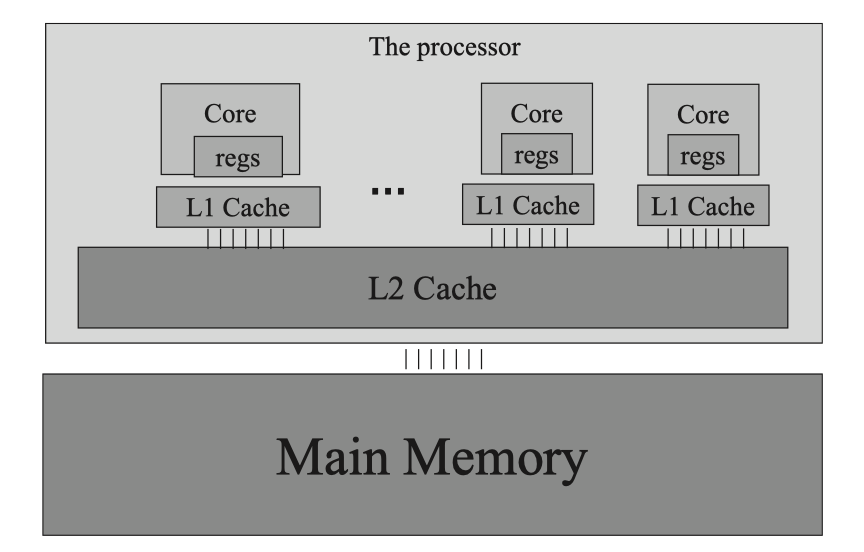
\includegraphics[width=0.9\textwidth]{figs/F7.10.png}
	\caption{\textit{使用指定用法创建访问器 }}
\end{figure}

让我们以前面的示例为例,重写它以添加扣除标签。 这个新的改进示例如图 7-10 所示。

我们首先声明Buffer,如图 7-8 所示。 我们还创建了稍后将使用的占位符访问器。 
现在让我们看看提交到队列的第一个任务。 之前,我们通过传递对Buffer的引用和命令组的处理程序对象来创建访问器。 
现在,我们向构造函数调用添加两个额外的参数。 第一个新参数是扣除标签。 
由于该Kernel正在为Buffer写入初始值,因此我们使用 write\_only 推导标签。 
这让运行时知道该Kernel正在生成新数据并且不会从Buffer读取。

第二个新参数是一个可选的访问器属性,类似于我们在本章前面看到的Buffer的可选属性。 
我们传递的属性 no\_init 让运行时知道可以丢弃Buffer的先前内容。 这很有用,因为它可以让运行时消除不必要的数据移动。 
在此示例中,由于第一个任务是写入Buffer的初始值,因此运行时无需在Kernel执行之前将未初始化的主机内存复制到设备。 
no\_init 属性对于本例很有用,但不应该用于读取-修改-写入的情况或仅更新Buffer中的某些值的Kernel。

我们提交到队列的第二个任务与之前相同,但现在我们向访问器添加推导标签。 
在这里,我们将标签 read\_only 添加到访问器 aA 和 aB 中,让运行时知道我们只会通过这些访问器读取Buffer A 和 B 的值。 
第三个访问器 aC 获得 read\_write 推导标签,因为我们将 A 和 B 的元素之和累加到 C 中。
我们在示例中显式使用该标签以保持一致,但这是不必要的,因为默认访问模式是 read\_write。

在我们使用占位符访问器的第三个任务中保留了默认用法。 这与我们在图 7-8 中看到的简化示例保持不变。 
我们的最终访问器(主机访问器结果)现在在创建时会收到一个推导标签。 
由于我们只读取主机上的最终值,因此我们将 read\_only 标记传递给构造函数。 
如果我们以破坏主机访问器的方式重写程序,则启动另一个对Buffer C 进行操作的Kernel将不需要将其写回设备,
因为 read\_only 标记让运行时知道它不会被 主人。

\subsubsection{我们可以用访问器做什么?}
使用访问器对象可以完成许多事情。 然而,我们能做的最重要的事情是在访问者的名字中拼写出来——访问数据。 
这通常是通过访问器的 [] 运算符之一完成的。 我们在图 7-8 和 7-10 的示例中使用 [] 运算符。 
该运算符采用可以正确索引多维数据的 id 对象或单个 size\_t。 当访问器具有多个维度时,可以使用第二种情况。 
在这种情况下,它返回一个对象,然后用 [] 再次索引该对象,直到我们到达标量值,在二维情况下,该对象的形式为 a[i][j]。 
请记住,访问器维度的排序遵循 C++ 的约定,其中最右边的维度是单位步幅维度(迭代“最快”)。

访问器还可以返回指向基础数据的指针。 可以按照正常的 C++ 规则直接访问该指针。 
请注意,该指针的地址空间可能会涉及额外的复杂性。

许多东西也可以从访问器对象中查询。 
示例包括通过访问器可访问的元素数量、它所覆盖的Buffer区域的大小(以字节为单位)或可访问的数据范围。

访问器提供了与 C++ 容器类似的接口,并且可以在许多可以传递容器的情况下使用。 
访问器支持的容器接口包括 data 方法(相当于 get\_pointer)以及多种向前和向后迭代器。

\subsection{总结}
在本章中,我们学习了Buffer和访问器。 Buffer是数据的抽象,它向程序员隐藏了内存管理的底层细节。 
他们这样做是为了提供更简单、更高层次的抽象。 
我们通过几个示例向我们展示了构建Buffer的不同方法以及可以指定以改变其行为的不同可选属性。 
我们学习了如何使用主机内存中的数据初始化Buffer,以及如何在使用完Buffer后将数据写回主机内存。

由于我们无法直接访问Buffer,因此我们学习了如何使用访问器对象来访问Buffer中的数据。 
我们了解了设备访问器和主机访问器之间的区别。 
我们讨论了不同的访问模式和目标,以及它们如何通知运行时程序将如何以及在何处使用访问器。 
我们展示了使用默认访问模式和目标来使用访问器的最简单方法,并且我们学习了如何区分占位符访问器和非占位符访问器。 
然后,我们了解了如何通过向访问器声明添加推导标签来为运行时提供有关访问器使用情况的更多信息,从而进一步优化示例程序。 
最后,我们介绍了在程序中使用访问器的许多不同方式。

在下一章中,我们将更详细地了解运行时如何使用我们通过访问器提供的信息来调度不同Kernel的执行。 
我们还将看到此信息如何通知运行时何时以及如何需要在主机和设备之间复制Buffer中的数据。 
我们将学习如何显式控制涉及Buffer的数据移动以及 USM 分配。